
% erstellt mit https://www.mathcha.io/editor

\tikzset{every picture/.style={line width=0.75pt}} %set default line width to 0.75pt        
\begin{center}
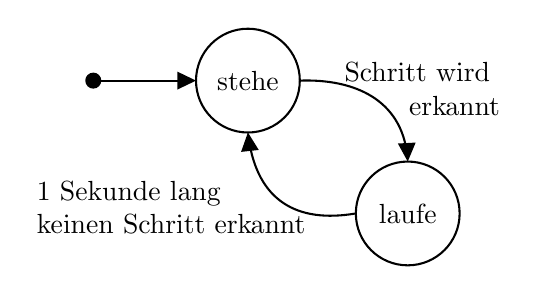
\begin{tikzpicture}[x=0.75pt,y=0.75pt,yscale=-1,xscale=1]
%uncomment if require: \path (0,410.90625); %set diagram left start at 0, and has height of 410.90625

%Shape: Circle [id:dp6318133684241805] 
\draw   (137,259) .. controls (137,245.19) and (148.19,234) .. (162,234) .. controls (175.81,234) and (187,245.19) .. (187,259) .. controls (187,272.81) and (175.81,284) .. (162,284) .. controls (148.19,284) and (137,272.81) .. (137,259) -- cycle ;
%Straight Lines [id:da6926894193378876] 
\draw    (87.5,259) -- (134,259) ;
\draw [shift={(137,259)}, rotate = 180] [fill={rgb, 255:red, 0; green, 0; blue, 0 }  ][line width=0.08]  [draw opacity=0] (8.93,-4.29) -- (0,0) -- (8.93,4.29) -- cycle    ;
\draw [shift={(87.5,259)}, rotate = 0] [color={rgb, 255:red, 0; green, 0; blue, 0 }  ][fill={rgb, 255:red, 0; green, 0; blue, 0 }  ][line width=0.75]      (0, 0) circle [x radius= 3.35, y radius= 3.35]   ;
%Shape: Circle [id:dp0026005274455069838] 
\draw   (214,323) .. controls (214,309.19) and (225.19,298) .. (239,298) .. controls (252.81,298) and (264,309.19) .. (264,323) .. controls (264,336.81) and (252.81,348) .. (239,348) .. controls (225.19,348) and (214,336.81) .. (214,323) -- cycle ;
%Curve Lines [id:da24747493565188639] 
\draw    (187,259) .. controls (213.54,258.07) and (235.88,268.28) .. (238.76,295.02) ;
\draw [shift={(239,298)}, rotate = 267.04] [fill={rgb, 255:red, 0; green, 0; blue, 0 }  ][line width=0.08]  [draw opacity=0] (8.93,-4.29) -- (0,0) -- (8.93,4.29) -- cycle    ;

%Curve Lines [id:da49971886799260323] 
\draw    (214,323) .. controls (185.38,327.88) and (166.65,316.74) .. (162.36,286.83) ;
\draw [shift={(162,284)}, rotate = 443.77] [fill={rgb, 255:red, 0; green, 0; blue, 0 }  ][line width=0.08]  [draw opacity=0] (8.93,-4.29) -- (0,0) -- (8.93,4.29) -- cycle    ;


% Text Node
\draw (239,323) node   [align=left] {laufe};
% Text Node
\draw (162,259) node   [align=left] {stehe};
% Text Node
\draw (246,263.04) node  [font=\normalsize] [align=left] {Schritt wird\\ \ \ \ \ \ \ \ erkannt};
% Text Node
\draw (125,320.04) node  [font=\normalsize] [align=left] {1 Sekunde lang \\keinen Schritt erkannt};


\end{tikzpicture}
\end{center}
